\documentclass[iop]{emulateapj}

\shorttitle{Fast Template Periodogram}
\shortauthors{Hoffman and VanderPlas 2016}
\usepackage{amsmath}
\newcommand{\todo}[1]{{\bf #1}}
\newcommand{\bigO}{\mathcal{O}}
\newcommand{\savg}[1]{\left<#1\right>}
\newcommand{\svar}{{\rm Var}}
\newcommand{\scov}{{\rm Cov}}
\newcommand{\Mshft}{\mathbf{M}_{\theta_2}}
\newcommand{\dMshft}{\partial\Mshft}
\newcommand{\dA}{\partial A}
\newcommand{\dB}{\partial B}



\begin{document}

\title{Fast and accurate template fitting with template periodograms}
\author{J. Hoffman}
\affil{Department of Astrophysical Sciences, Princeton University, Princeton NJ 08540}
\email{jah5@princeton.edu}

\author{J. VanderPlas}
\affil{eScience Institute, University of Washington, Seattle, WA 98195}
\email{jakevdp@cs.washington.edu}

\author{J. Hartman}
\affil{Department of Astrophysical Sciences, Princeton University, Princeton NJ 08540}
\email{jhartman@astro.princeton.edu}

\author{G. Bakos}
\affil{Department of Astrophysical Sciences, Princeton University, Princeton NJ 08540}
\email{gbakos@astro.princeton.edu}

\begin{abstract}
    Astrophysical time series often contain periodic signals. In the near future,
    the sheer volume of astrophysical time series data (e.g. from LSST) will demand
    computationally efficient methods for detecting and characterizing such signals. 
    The most efficient algorithms that exist to date are those that exploit the $\bigO(N\log N)$ nature of
    the Fast Fourier Transform. However, these methods are not optimal for non-sinusoidal
    signal shapes. Template fitting optimizes sensitivity for \emph{a priori} known
    signal shapes but at enormous computational cost that scales as $\bigO(N^2)$, and without the garauntee
    that the fitting procedure obtains the best fit at each trial frequency. In this work, we present
    a non-linear extension of the Lomb-Scargle periodogram as a template-fitting
    algorithm that is both accurate (the exact optimal solutions are obtained except
    in rare cases) and computationally efficient (scaling as $\bigO(N\log N)$). We show that our method
    is twice as fast as existing algorithms for small problems ($N\lesssim 10$ observations) and
    up to 3 orders of magnitude faster for long base-line time series with $N\sim 10^4$ 
    observations. Additional speedups are likely with improvements to the existing implementation.
\end{abstract}

\section{Introduction}\label{sec:introduction}

Astrophysical time series are challenging to analyze. Unlike
time series in other domains like economics and finance, astrophysical 
observations are often irregularly sampled in time with heteroskedastic, 
non-Gaussian, and time-correlated measurement uncertainties.

Irregular sampling thwarts the straightforward application of many well-known 
time series tools like the discrete Fourier transform (DFT) and the auto-regressive 
moving average (ARMA) models. The DFT is a particularly unfortunate loss, since
the Fast Fourier Transform \citep{Cooley+Tukey_1965} reduces the $\bigO(N^2)$ DFT
to $\bigO(N\log N)$, and is a powerful tool for finding periodic signals.

Fortunately, the DFT can be extended to irregularly sampled data via what is sometimes
referred to as the classical periodogram \citep{Stoica+Li+He_2009}

\begin{equation}
    P_x(\omega) = \frac{1}{N^2}\left|\sum_{n=0}^{N - 1} y_n e^{- i \omega t_n}\right|^2.
\end{equation}

However, as \cite{Stoica+Li+He_2009} point out, this is not an
optimal measure of periodicity. A more robust estimate of the power spectrum is
given by the Lomb-Scargle periodogram \citep{Lomb_1976,Scargle_1982,Barning_1963,Vanicek_1971}.

ARMA models can also be extended to unevenly sampled data with the CARMA
model \citep{Kelly_etal_2014, Zinn_etal_2016}, but for the purposes of this paper, 
we focus solely on tools applicable to the detection of periodic signals in astrophysical data. 

The Lomb-Scargle periodogram and its extensions can be expressed in terms of 
least-squares minimization between the data $\{y_n\}_{n=1}^N$ and a model $\hat{y}$.
In the original formulation of the Lomb-Scargle periodogram, 

\begin{equation}
    \hat{y}_{\rm LS}(t|\theta, \omega) = \theta_0\cos{\omega t} + \theta_1\sin{\omega t}.
\end{equation}

This is equivalent to performing a DFT if the data is regularly sampled. The Lomb-Scargle
periodogram can be obtained from solving the linear system of equations that arise from
the condition that the summed squares of residuals between the data and the optimal
model,

\begin{equation}
\chi^2(\theta, S) \equiv \sum_i (y_i - \hat{y}(t_i|\theta) )^2,
\end{equation}

\noindent must be a local minimum. This means that

\begin{equation}
    \left.\frac{\partial\chi^2}{\partial\theta_i}\right|_{\theta=\theta_{\rm best}} = 0~~\forall\theta_i\in\theta.
\end{equation}

The resulting periodogram can be expressed as

\begin{equation}
\begin{split}
    P_{\rm LS} = \frac{1}{2\sigma^2}&\left(\frac{\left[\sum_{n=1}^N (y_n - \bar{y})\cos{\omega t_n}\right]^2}{\sum_{n=1}^N \cos^2{\omega t_i}} \right. \\
                &\left.+ \frac{\left[\sum_{n=1}^N (y_n - \bar{y})\sin{\omega t_n}\right]^2}{\sum_{n=1}^N \sin^2{\omega t_i}} \right),
\end{split}
\end{equation}

\noindent where $\bar{y} = \mathbb{E}[y_n]$, the mean of the data, and 
$\sigma = {\rm Var}(y_n)$, the variance of the data. 

Heteroskedasticity can be handled by using weighted least squares, 

\begin{equation}
\chi^2(\theta, S) \equiv \sum_i \frac{(y_i - \hat{y}(t_i|\theta) )^2}{\sigma_i}^2,
\end{equation}

\noindent with weights $w_i = \frac{W}{\sigma_i^2}$, $W\equiv\sum \sigma_i^{-2}$ being
a normalization factor to ensure $\sum w_i = 1$, and correlated uncertainties
can be accounted for by using the full covariance matrix, $\Sigma_{ij} = {\rm Cov}\left((y_i - \bar{y})(y_j - \bar{y})\right)$.

\begin{equation}
\chi^2(\theta, S) \equiv (y_i - \hat{y}(t_i|\theta) )^{\rm T}\Sigma(y_i - \hat{y}(t_i|\theta) ).
\end{equation}

If we assume the covariance matrix is diagonal, the Lomb-Scargle periodogram can be
evaluated quickly in one of two popular ways. The first, by \cite{Press+Rybicki_1989}
involves``extirpolating'' irregularly sampled data onto a regularly sampled mesh,
and then performing FFTs to evaluate the necessary sums. The second, as pointed
out in \cite{Leroy_2012}, is to use the non-equispaced FFT (NFFT) \cite{NFFT} to evaluate
the sums; this provides an order of magnitude speedup over the \cite{Press+Rybicki_1989}
algorithm, and both algorithms scale as $\bigO(N\log N)$.

There also exists a continually growing number of alternative methods for detecting
periodic signals in astrophysical data. Some of these methods can reliably
outperform the Lomb-Scargle periodogram, especially for non-sinusoidal signal shapes
(see \cite{Graham_etal_2013} for a recent empirical review). However, a key advantage
that the LS periodogram and its extensions have over many alternatives is speed.
Virtually all other methods scale as $N\times N_f \sim N^2\sim N_f^2$, where $N$ is the number
of observations and $N_f$ is the number of trial frequencies, while the Lomb-Scargle
periodogram scales as $N_f\log N_f \sim N\log N$.

The importance of efficient algorithms will only become more important as the volume
of data produced by astronomical observatories continues to grow. The HATNet telescope,
for example, has already made $\bigO(10^4)$ observations of $\bigO(10^6-10^7)$ stars. 
The Gaia telescope \citep{GAIA} is set to produce $\bigO(10-100)$ observations of 
$\bigO(10^9)$ stars. The Large Synoptic Survey Telescope (LSST; \cite{LSST}) will 
produce 15 Terabytes of data per night once operation begins in 2023.

This paper develops new extensions to least-squares spectral analysis for arbitrary
signal shapes. For non-periodic signals this method is known as matched filter analysis,
and can be extended to search for periodic signals by phase folding the data
at different trial periods. We refer to latter technique, the subject of this paper, as
template fitting. 

Recently, \cite{Sesar_etal_2016} found that template fitting significantly improved
period and amplitude estimation for RR Lyrae in Pan-STARRS DR1 \citep{PanSTARRS}. Since the signal
shapes for RR Lyrae in various bandpasses are known \emph{a priori} (see \cite{Sesar_etal_2010}), 
template fitting provides an optimal estimate of amplitude and period,
given that the object is indeed an RR Lyrae star well modeled by at least one of the templates. 
Templates were especially crucial for Pan-STARRS data, since there are typically only 
35 observations per source over 5 bands \citep{Hernitschek_etal_2016}, not enough to obtain 
accurate amplitudes empirically by phase-folding. By including domain knowledge (i.e. knowledge of what RR Lyrae 
lightcurves look like), template fitting allows for accurate inferences of amplitude even 
for undersampled lightcurves.

However, the improved accuracy comes at substantial computational cost: the template fitting 
procedure took 30 minutes per CPU per object, and \cite{Sesar_etal_2016} were forced to limit
the number of fitted lightcurves ($\lesssim 1000$) in order to keep the computational costs
to a reasonable level. Several cuts were made before the template fitting step to reduce the
more than 1 million Pan-STARRS DR1 objects to a small enough number, and each of these steps
removes a small portion of RR Lyrae from the sample. Though this number was reported by
\cite{Sesar_etal_2016} to be small ($\lesssim 10\%$), it may be possible to further improve
the completeness of the final sample by applying template fits to a larger number of objects,
which would require either more computational resources, more time, or, ideally, a more efficient
template fitting procedure.

The paper is organized as follows. Section \ref{sec:derivations} poses the problem of template
fitting in the language of least squares spectral analysis and derives the fast template
periodogram. Section \ref{sec:implementation} describes a freely available implementation 
of the new template periodogram. Section \ref{sec:discussion} summarizes our results, 
addresses caveats, and discusses possible avenues for improving the efficiency of the current 
algorithm.


%Many astrophysical systems exhibit brightness fluctuations, and
%detecting these brightness fluctuations in data has been a challenge for astronomers for \todo{what was the
%earliest detection of variability?}. 

%Some of these variable systems, such as eclipsing binaries, transiting
%exoplanets, or pulsating stars, exhibit periodic brightness fluctuations. Powerful methods
%for detecting periodicities in observational data have been developed and deployed

%A plethora of astronomical systems exhibit periodic fluctuations
%in brightness. These systems are important for many reasons; pulsating
%stars are valuable laboratories for testing our understanding
%of stellar physics \todo{cite pulsating stars}, determining
%stellar composition \todo{cite astroseismology}, and as distance
%indicators \todo{cite distance indicators}. Transiting exoplanets
%are valuable 

\section{Derivations}\label{sec:derivations}

We define a template $\mathbf{M}$

\begin{equation}
    \mathbf{M} : [0, 1)\rightarrow\mathbb{R},
\end{equation}

\noindent as a mapping between the unit interval and the set of real numbers. We
restrict our discussion to sufficiently smooth templates such that
$\mathbf{M}$ can be adequately described by a truncated Fourier series

\begin{equation}
    \hat{\mathbf{M}}(\omega t|H) = \sum_{n=1}^H\left[c_n\cos{n\omega t} + s_n\sin{n\omega t}\right]
\end{equation}

\noindent for some $H > 0$. Specifically, we require that 

\begin{equation}
\begin{split}
    (\forall \epsilon > 0)&(\exists H \in \mathbb{N})~~{\rm s.t.}\\
    &\left|\mathbf{M}(t) - \hat{\mathbf{M}}(t|H)\right| < \epsilon~~\forall t\in [0, 1).
\end{split}
\end{equation}

We now construct a periodogram for this template. The periodogram assumes 
that an observed time series $S = \{(t_i, y_i, \sigma_i)\}_{i=1}^N$ can be modeled 
by a scaled, transposed template that repeats with period $2\pi / \omega$, i.e.

\begin{equation}
y_i \approx \hat{y}(\omega t_i|\theta, \mathbf{M}) = \theta_1\mathbf{M}(\omega t_i - \theta_2) + \theta_3,
\end{equation}

\noindent where $\theta\in \mathbb{R}^3$ is a set of model parameters. 

The optimal parameters are the location of a local minimum of the (weighted) sum of 
squared residuals,

\begin{equation}
    \chi^2(\theta, S) \equiv \sum_i w_i (y_i - \hat{y}(\omega t_i|\theta) )^2,
\end{equation}

\noindent and thus the following condition must hold for all three model parameters at 
the optimal solution $\theta=\theta_{\rm opt}$:

\begin{equation}\label{eq:chi2conds}
    \left.\frac{\partial\chi^2}{\partial\theta_i}\right|_{\theta=\theta_{\rm opt}} = 0~~\forall\theta_i\in\theta.
\end{equation}

Note that we have implicitly assumed $\chi^2(\theta,S)$ is a $C^1$ differentiable 
function of $\theta$, which requires that both $\mathbf{M}$ and $\mathbf{M}^2$ are 
$C^1$ differentiable functions. Though this assumption could be violated if we 
considered a more complete set of templates, (e.g. a box function), our restriction 
to truncated Fourier series guarantees that both $\mathbf{M}$ and $\mathbf{M}^2$ 
are $C^1$ differentiable and thus that $\chi^2(\theta,S)$ is $C^1$ differentiable.

We can derive a system of equations for $\theta_{\rm opt}$ from the condition given 
in Equation \ref{eq:chi2conds}. The explicit condition that must be met for each parameter $\theta_i$ is simplified below

\begin{equation}\label{eq:simpconds}
\begin{split}
0 &= \left.\frac{\partial\chi^2}{\partial\theta_i}\right|_{\theta=\theta_{\rm opt}}\\
  &= -2\sum_n w_n(y_n - \hat{y})\frac{\partial\hat{y}}{\partial \theta_i} \\
\sum_n w_ny_n\left(\frac{\partial\hat{y}}{\partial \theta_i}\right)_n &= \sum_n w_n \hat{y}_n \left(\frac{\partial\hat{y}}{\partial \theta_i}\right)_n.
\end{split}
\end{equation}

The above is a general result that extends to all least squares periodograms.
To hopefully make our derivations more intuitive, we adopt the following notation:

\begin{eqnarray}
\savg{X} &\equiv& \sum_n w_n X_n\\
\savg{XY} &\equiv& \sum_n w_n X_nY_n\\
\svar(X) &\equiv& \savg{X^2} - \left<X\right>^2\\
\scov(X, Y) &\equiv& \savg{XY} - \savg{X}\savg{Y}
\end{eqnarray}

In addition, we denote shifted template $\mathbf{M}(x - \theta_2)$ by $\Mshft(x)$.

For the amplitude and offset model parameters ($\theta_1$ and $\theta_3$, respectively), 
we obtain the following relations from Equation \ref{eq:simpconds}

\begin{eqnarray}
    \savg{y\Mshft(\omega t)} &=& \theta_1\savg{\Mshft^2(\omega t)} + \theta_3\savg{\Mshft(\omega t)}\\
    \theta_3 &=& \bar{y} - \theta_1\savg{\Mshft(\omega t)}.
\end{eqnarray}

Combining these expressions yields

\begin{equation}\label{eq:th13eq}
\theta_1 = \frac{\savg{(y - \bar{y})\Mshft(\omega t)}}{\svar(\Mshft(\omega t))}.
\end{equation}

For the offset parameter $\theta_2$, 

\begin{equation}
 \begin{split}
     \frac{\partial\hat{y}}{\partial\theta_2} &= \theta_1\frac{\dMshft}{\partial\theta_2}\\
     &= -\theta_1\dMshft,
 \end{split}
\end{equation}

\noindent where 

\begin{equation}
 \dMshft(x) = \sum_n \left[s_n\cos{n(x - \theta_2)} - c_n\sin{n(x - \theta_2)}\right].
\end{equation}
 
From this we obtain

\begin{equation}\label{eq:th2eq}
 \theta_1 = \frac{\savg{(y - \bar{y})\dMshft(\omega t)}}{\scov\left(\Mshft(\omega t),\dMshft(\omega t)\right)},
\end{equation}

\noindent which, combined with Equation \ref{eq:th13eq}, provides 
a non-linear expression for $\theta_2$:

\begin{equation}\label{eq:th2cond}
\begin{split}
&\savg{(y - \bar{y})\dMshft(\omega t)}\svar(\Mshft(\omega t)) \\
 &= \savg{(y - \bar{y})\Mshft(\omega t)}\scov(\Mshft(\omega t),\dMshft(\omega t)).
\end{split}
\end{equation}

To obtain an explicit expression for Equation \ref{eq:th2cond},
we define several quantities, 

\begin{eqnarray}
CC_{nm} &\equiv& \scov(\cos{n\omega t},\cos{m\omega t})\label{eq:CCdef}\\
CS_{nm} &\equiv& \scov(\cos{n\omega t},\sin{m\omega t})\label{eq:CSdef}\\
SS_{nm} &\equiv& \scov(\sin{n\omega t},\sin{m\omega t})\label{eq:SSdef}\\
YC_n &\equiv& \savg{(y - \bar{y})\cos{n\omega t}}\label{eq:YCdef}\\
YS_n &\equiv& \savg{(y - \bar{y})\sin{n\omega t}}\label{eq:YSdef},
\end{eqnarray}

\noindent all of which can be evaluated efficiently with NFFTs. We also obtain
an expression for the shifted template:

\begin{equation}
\begin{split}
    \Mshft(x) &= \sum_n \left[c_n\cos{n(x - \theta_2)} + s_n\sin{n(x - \theta_2)}\right]\\
    %\Mshft(x) &= \sum_n \left[c_n\left(\cos{nx}\cos{n\theta_2} + \sin{nx}\sin{n\theta_2}\right)\right. \\
    %        &\qquad\quad\left. + s_n\left(\sin{nx}\cos{n\theta_2} - \cos{nx}\sin{n\theta_2}\right)\right]\\
    \Mshft(x) &= \sum_n \left[\left(c_n\cos{n\theta_2} - s_n\sin{n\theta_2}\right)\cos{nx} \right.\\
              &\qquad\quad \left. + \left(s_n\cos{n\theta_2} + c_n\sin{n\theta_2}\right)\sin{nx}\right]\\
    \Mshft(x) &= \sum_n \left[\left(c_nT_n(u) \mp s_n\sqrt{1 - u^2}U_{n-1}(u)\right)\cos{nx} \right.\\
              &\qquad\quad \left. + \left(s_nT_n(u) \pm c_n\sqrt{1 - u^2}U_{n-1}(u)\right)\sin{nx}\right]\\
    \Mshft(x) &= \sum_n \left[A_n(u)\cos{nx} + B_n(u)\sin{nx}\right]
\end{split}
\end{equation}

\noindent where $u \equiv \cos \theta_2$, $T_n$ and $U_n$ are the Chebyshev polynomials 
of the first and second kind, respectively, and the $\pm$ ambiguity arises out of the
two possible signs for $\sin{\theta_2}$.

The derivatives of first and second order Chebyshev polynomials are known to be

\begin{eqnarray}
\frac{dT_n}{dx} &=& nU_{n-1}(x)\\
\frac{dU_n}{dx} &=& \frac{(n+1)T_{n+1}(x) - xU_n(x)}{x^2 - 1},
\end{eqnarray}

\noindent and this implies that the first derivative of the shifted template is

\begin{equation}
\begin{split}
\dMshft(x) &= \sum_n \left[n\left(c_nU_{n-1}(u) \pm s_n\frac{T_n(u)}{\sqrt{1 - u^2}}\right)\cos{nx} \right.\\
           &\qquad\quad \left. + n\left(s_nU_{n-1}(u) \mp c_n\frac{T_n(u)}{\sqrt{1 - u^2}}\right)\sin{nx}\right]\\
\dMshft(x) &= \sum_n \left[\dA_n(u) \cos{nx} + \dB_n(u) \sin{nx}\right]
\end{split}
\end{equation}

Using the sums provided in Equations \ref{eq:CCdef} -- \ref{eq:YSdef}, writing 
$A_n$ and $B_n$ as as shorthand for $A_n(u)$ and $B_n(u)$, and employing 
Einstein summation notation, we have that

\begin{align}
\savg{(y - \bar{y})\Mshft} &= A_n YC^n + B_n YS^n\\
\savg{(y - \bar{y})\dMshft} &= \dA_n YC^n + \dB_n YS^n\\
\svar(\Mshft^2) &= 
\begin{aligned}[t]
&A_nA_m CC^{nm} \\
& + 2A_nB_m CS^{nm}
+ B_nB_m SS^{nm}
\end{aligned}\\
\scov(\Mshft, \dMshft) &=
\begin{aligned}[t]
&A_n \dA_m CC^{nm}\\
&+ (A_n\dB_m + B_n \dA_m)CS^{nm} \\
&+ B_n\dB_m SS^{nm}
\end{aligned}.
\end{align}

Equation \ref{eq:th2cond} now becomes

%\begin{widetext}
\begin{align}\label{eq:polynomial}
0 &= 
\begin{aligned}[t]
&\quad A_iA_j\dA_k\left(YC^iCC^{jk} -  YC^kCC^{ji}\right)\\
&+ A_iA_j\dB_k\left(YC^iCS^{jk} - YS^kCC^{ji}\right)\\
&+ A_iB_j\dA_k\left(YC^iCS^{kj} + YS^jCC^{ki}\right)\\
&+ A_iB_j\dB_k\left(YC^iSS^{jk} + YS^jCS^{ik}\right)\\
&+ B_iB_j\dA_k\left(YS^iCS^{kj} - YC^kSS^{ij}\right)\\
&+ B_iB_j\dB_k\left(YS^iSS^{jk} - YS^kSS^{ji}\right).
\end{aligned}
\end{align}
%\end{widetext}

Each $AA\dA$, $AA\dB$, ..., $BB\dB$ can be expressed as 

\begin{equation}
AA\dA,~AA\dB,~...= p(u) \pm (1 - u^2)^{-1/2}q(u),
\end{equation}

\noindent where both $p(u)$ and $q(u)$ are polynomials in $u$. Therefore, Equation
\ref{eq:polynomial} can be expressed as

\begin{equation}
0 = (1 - u^2)\hat{p}^2(u) - \hat{q}^2(u) = \hat{P}(u)
\end{equation}

\noindent for some polynomials $\hat{p}, \hat{q}$, and $\hat{P}$.


We have derived an explicit, non-linear system of equations to solve for
the parameters $\theta_1$, $\theta_2$, and $\theta_3$. Solving this system of equations
requires finding the zeros of a polynomial $\hat{P}(u)$ at the given trial frequency.

\subsection{Extending to multi-band observations}

As shown in \cite{Vanderplas+Ivezic_2015}, the multi-phase periodogram (their 
$(N_{\rm base}, N_{\rm band}) = (0, 1)$ periodogram), for any model can
be expressed as a linear combination of single-phase periodograms:

\begin{equation}
\label{eq:multiband}
P^{(0,1)} = \frac{\sum_{k=1}^K\chi^2_{0, k}P_{k}}{\sum_{k=1}^K\chi^2_{0,k}}
\end{equation} 

\noindent where $K$ denotes the number of bands. This means that the template
periodogram can be applied to multi-band time series, which is crucial for
experiments like LSST, SDSS, Pan-STARRS, and other current and future surveys.




\subsection{Computational requirements}

For a given number of harmonics $H$, the task of deriving 
$\hat{P}$ requires a triple sum over $H$ terms, with each sum
requiring $\bigO(n_{\hat{P}})$ operations, where $n_{\hat{P}}$ is the order
of $\hat{P}$. The order of $\hat{P}$ can be shown to be

\begin{equation}
6H - {\rm gcf}\left((1 - u^2)\star\hat{p}^2, \hat{q}^2\right) \propto H,
\end{equation}

\noindent where ${\rm gcf}(p_1, p_2)$ denotes the greatest common polynomial factor
between polynomials $p_1$ and $p_2$. Computing the coefficients of $\hat{P}$ therefore
scales as $\bigO(H^4)$ at each trial frequency. 

The computational complexity of polynomial root finding
is algorithm dependent. If we choose to perform singular value decomposition of
the polynomial companion matrix\footnote{The \texttt{numpy.polynomial.polyroots} 
function uses this method.}, the root finding step scales as 
$\bigO(n_{\hat{P}}^3) = \bigO(H^3)$. The polynomial root-finding step 
should be asymptotically faster (for large $H$) than the computation of 
the polynomial coefficients.

When considering $N_f$ trial frequencies, the polynomial computation and root-finding 
step scales as $\bigO(H^4N_f)$. The computation of the sums 
(Equations \ref{eq:CCdef} -- \ref{eq:YSdef}) scales as $\bigO(HN_f\log HN_f)$.
Therefore, the entire template periodogram scales as 

\begin{equation}
\bigO(HN_f \log HN_f + H^4N_f).
\end{equation}

\begin{figure}
    \centering
    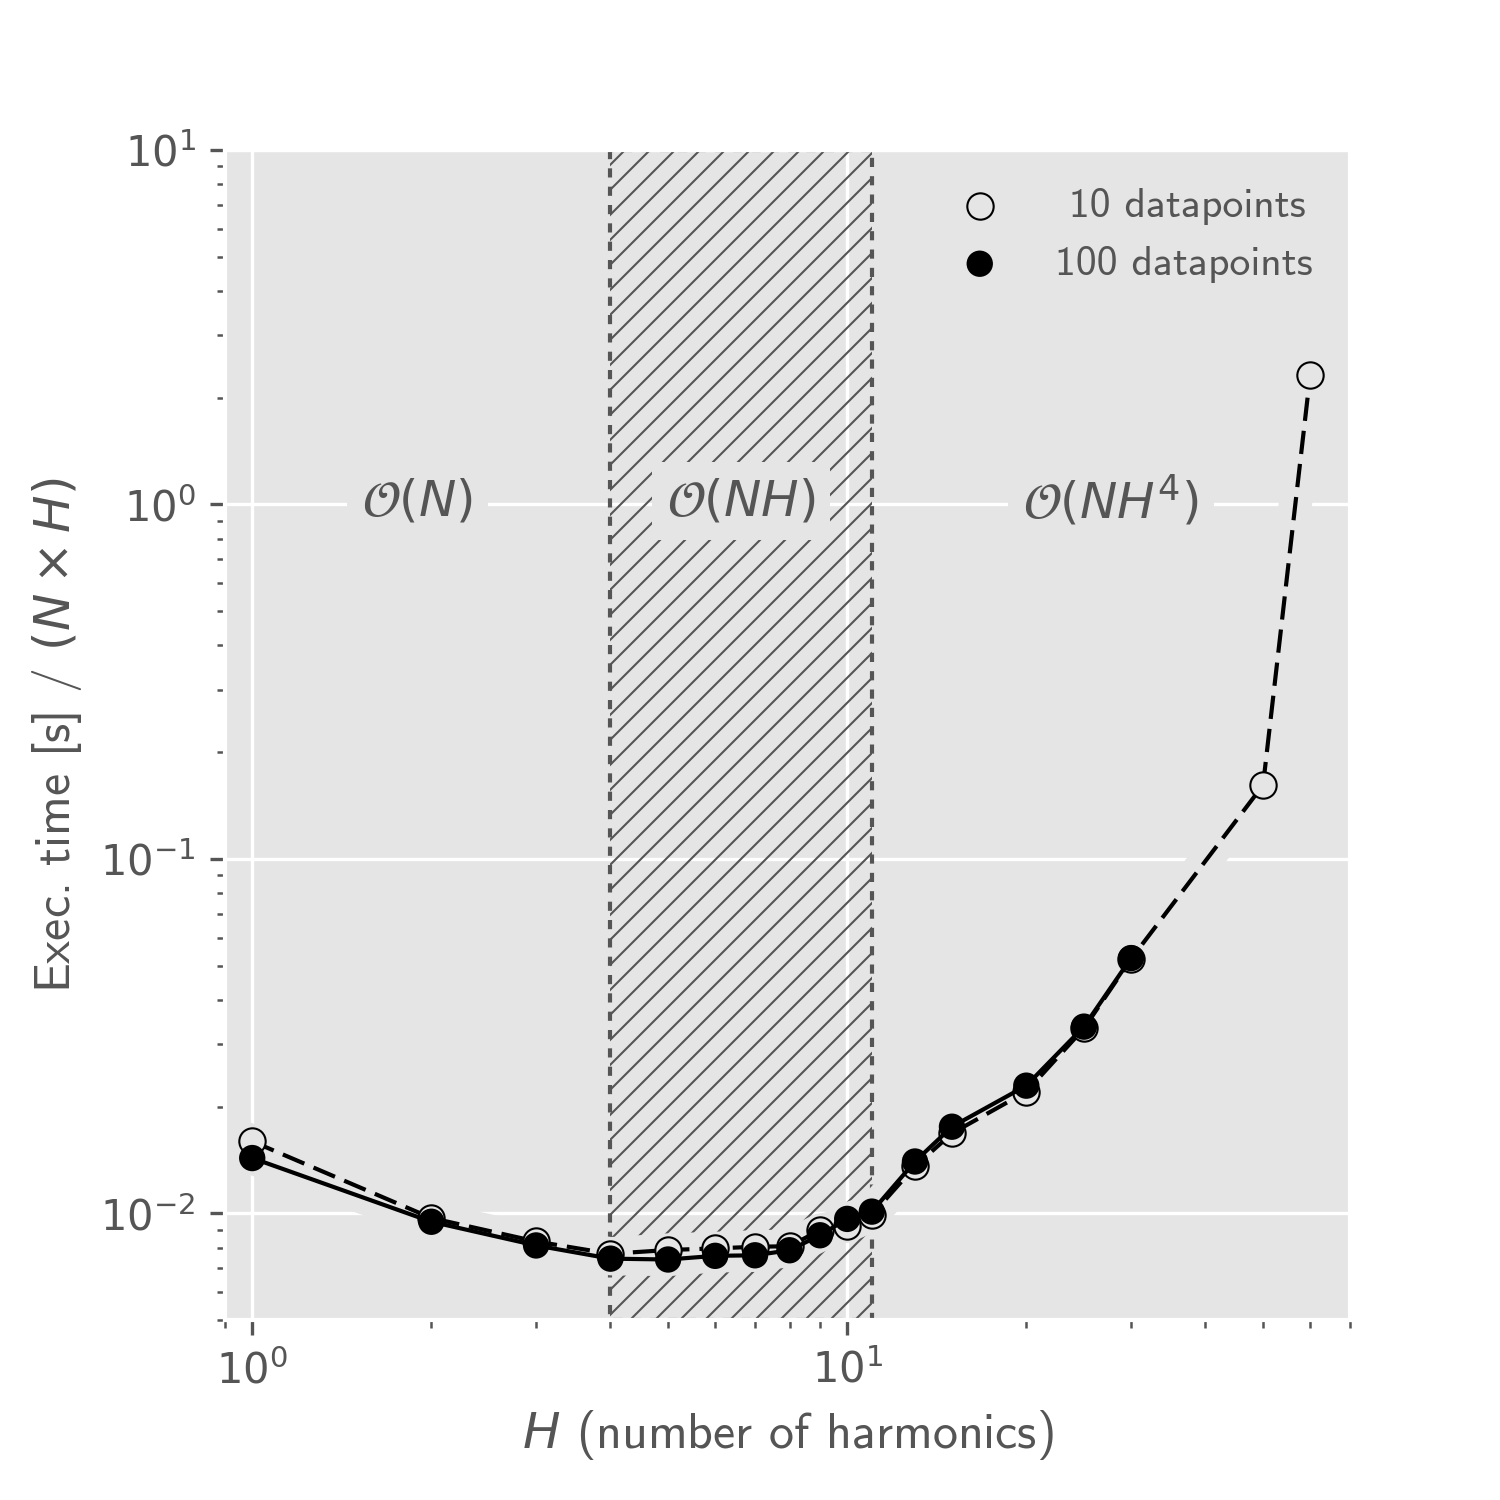
\includegraphics[width=0.5\textwidth]{plots/timing_vs_nharm.png}
    \caption{\label{fig:timingnharm} Computation time of FTP scaled by $NH$ for
            different numbers of harmonics. For $H\lesssim 3$, FTP scales
            sublinearly in $H$ (possibly due to a constant overhead per
            trial frequency, independent of $H$). When $3 \lesssim H \lesssim 11$,
            FTP scales approximately linearly in $H$, and when $H \gtrsim 11$
            FTP approaches the $\bigO(H^4)$ scaling limit.}
\end{figure}

For a fixed number of harmonics $H$, the template periodogram scales as
$\bigO(N_f\log N_f)$. However, for a constant number of trial frequencies $N_f$, 
the template algorithm scales as $\bigO(H^4)$, and computational resources
alone limit $H$ to reasonably small numbers $H\lesssim15$ (see Figure \ref{fig:timingnharm}).


\section{Implementation}\label{sec:implementation}

\begin{figure*}
    \centering
    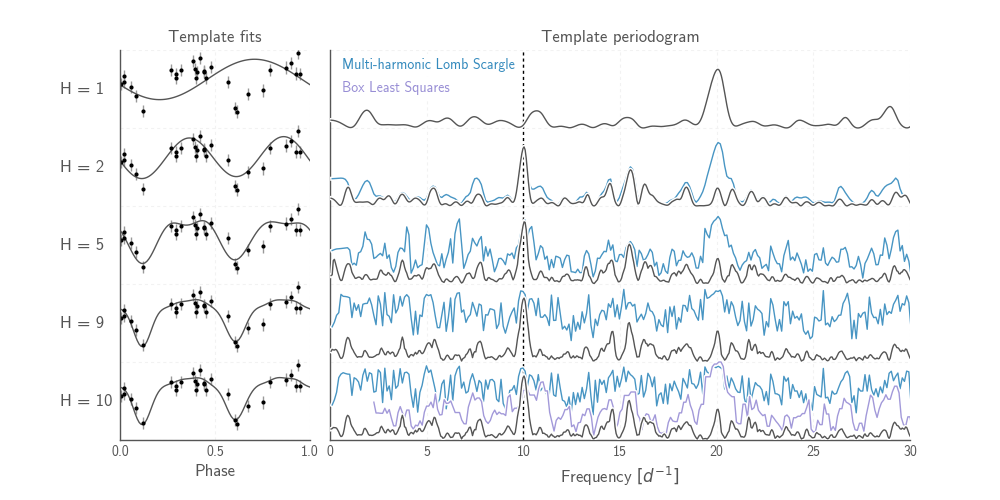
\includegraphics[width=\textwidth]{plots/templates_and_periodograms.png}
    \caption{\label{fig:tempsandpdgs} Template periodograms performed on a simulated eclipsing
            binary lightcurve (shown phase-folded in the left-hand plots). The top-most plot 
            uses only one harmonic, equivalent to a Lomb-Scargle periodogram. Subsequent plots
            use an increasing number of harmonics, which produces a narrower and higher peak
            height around the correct frequency. For comparison, the multi-harmonic extension 
            to Lomb-Scargle is plotted in blue, using the same number of harmonics as the FTP.
            The Box Least-Squares \citep{Kovacs_2002} periodogram is shown in the final plot.}
\end{figure*}

An open-source implementation of the template periodogram in Python is
available.\footnote{\url{https://github.com/PrincetonUniversity/FastTemplatePeriodogram}} 
Computing $\hat{P}(u)$ is done using the \texttt{numpy.polynomial} module 
\citep{Scipy}. The \texttt{pynfft} Python module,
\footnote{https://pypi.python.org/pypi/pyNFFT} which provides a Python 
wrapper for the NFFT library \citep{NFFT}, is used to compute the necessary 
sums for a particular time series.

No explicit parallelism is used anywhere in the current implementation, 
however the NFFT library optionally exploits OpenMP if compiled
to do so (requires specifying the \texttt{--enable-openmp} flag
when running \texttt{configure}) and certain linear algebra operations
in \texttt{Scipy} may use OpenMP via calls to BLAS libraries that
have OpenMP enabled.

All timing tests were run on a quad-core 2.6 GHz Intel Core i7 MacBook 
Pro laptop (mid-2012 model) with 8GB of 1600 MHz DDR3 memory. The NFFT
library (version 3.2.4) was compiled with \texttt{--enable-openmp}, and
the \texttt{Scipy} stack (version 0.18.1) was compiled with multi-threaded MKL libraries.
However, the slowest portion of the algorithm, computing the polynomial
coefficients, uses the \texttt{numpy.einsum} function which is not
multi-threaded. 

\subsection{Comparison with \texttt{gatspy}}

The \texttt{gatspy} (General tools for Astronomical Time Series in Python; 
\cite{gatspy,Vanderplas+Ivezic_2015}) library provides template fitting
routines, which rely on non-linear optimization at each trial frequency
to pick the optimal parameters $\theta$. We compare the accuracy and
speed of the fast template periodogram with the template fitting
procedure provided by the \texttt{gatspy} library.

Periodograms computed in Figures \ref{fig:tempsandpdgs}, \ref{fig:corrwgats},
and \ref{fig:corrwhighh} used simulated data. The simulated data has uniformly
random observation times, with gaussian-random, homoskedastic, uncorrelated 
uncertainties. An eclipsing binary template, generated by fitting an
eclipsing binary in the HATNet dataset (\todo{put in HATID for template})
with a 10-harmonic truncated Fourier series.

\subsubsection{Accuracy}

\begin{figure*}
    \centering
    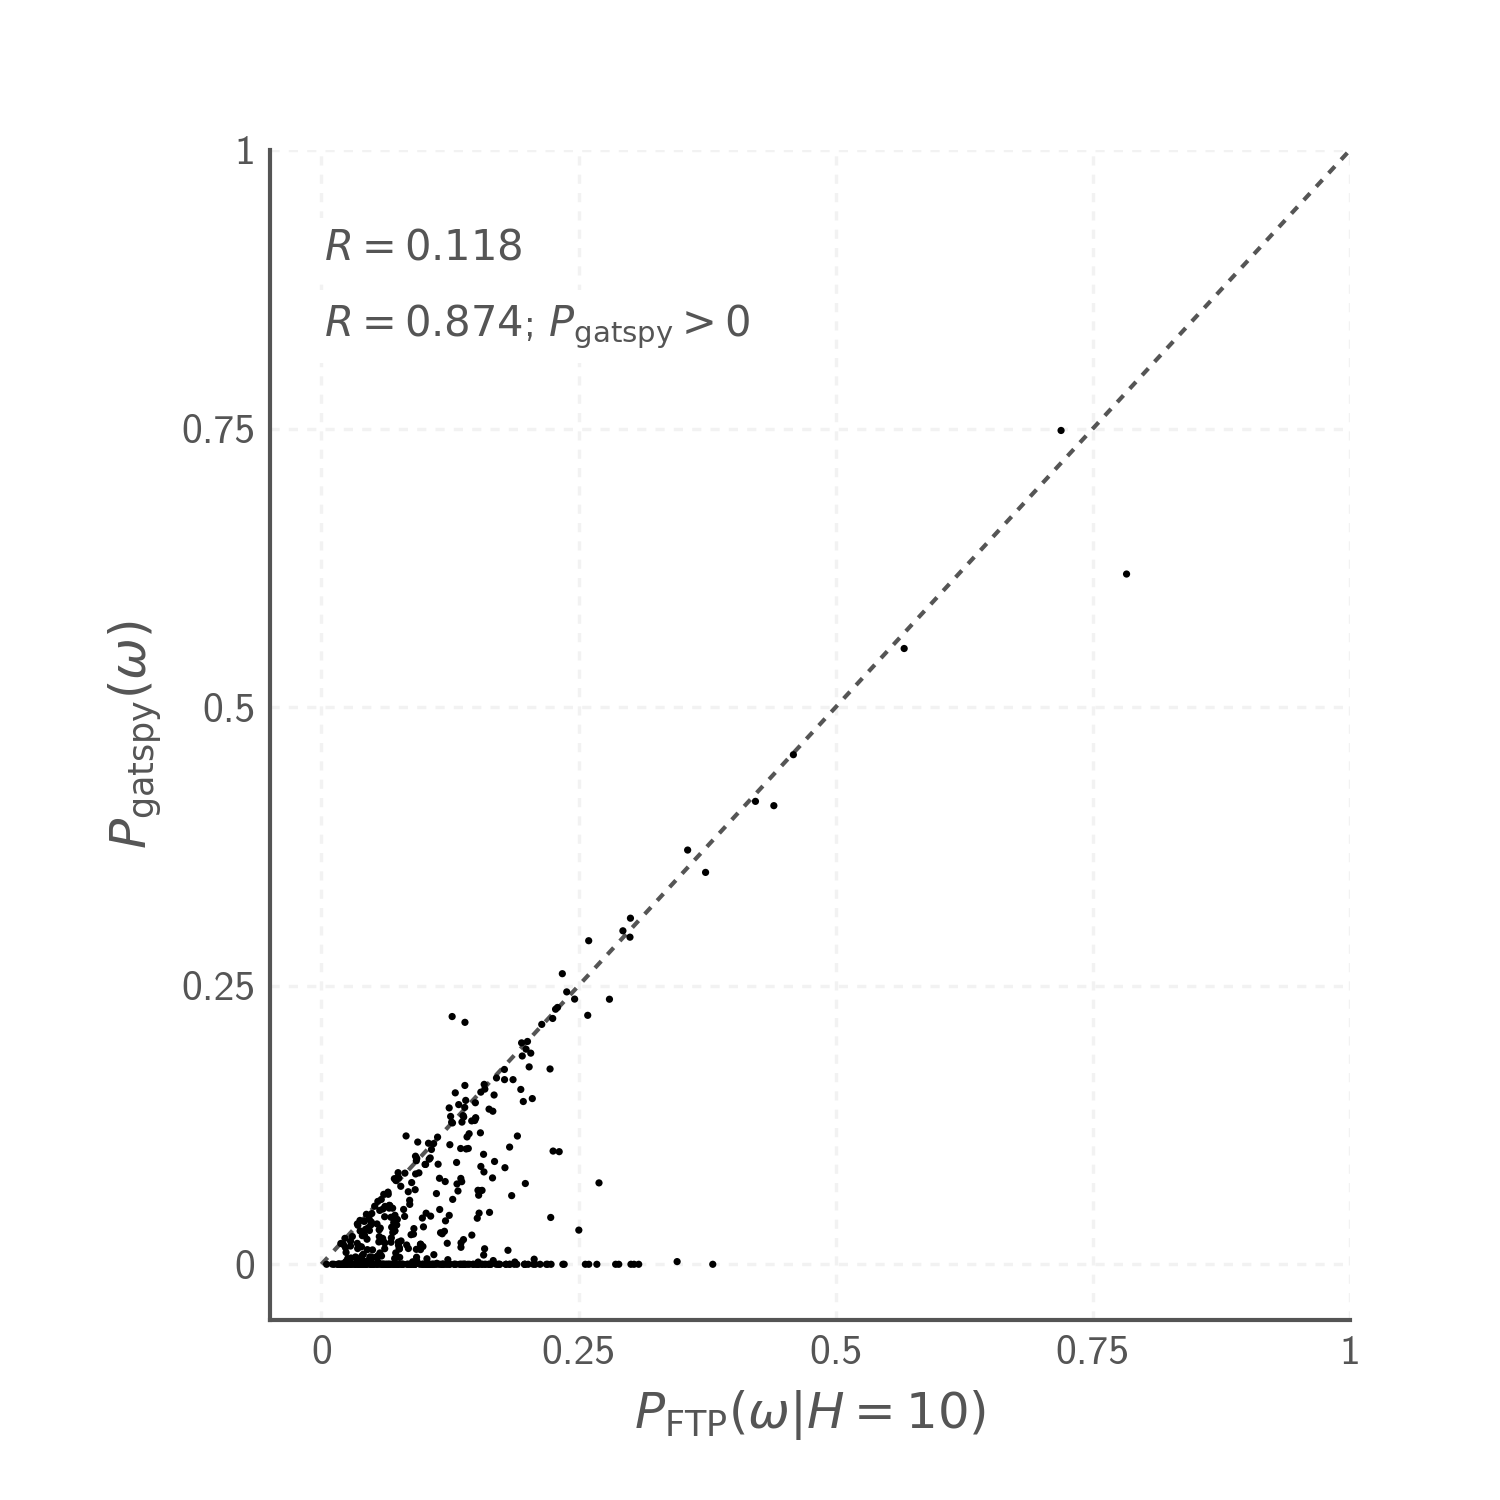
\includegraphics[width=\textwidth]{plots/correlation_with_gatspy.png}
    \caption{\label{fig:corrwgats} Comparing the gatspy template periodogram with 
            the FTP using the same simulated data as shown in Figure \ref{fig:tempsandpdgs}.
            When $H$ is sufficiently large, FTP consistently finds more optimal template
            fits than Gatspy. Gatspy numerically minimizes the $\chi^2$ at each frequency,
            and sometimes gets caught in a local minimum. The FTP solves for the optimal
            fit parameters directly, and therefore is able to achieve greater accuracy than Gatspy.}
\end{figure*}

\begin{figure*}
    \centering
    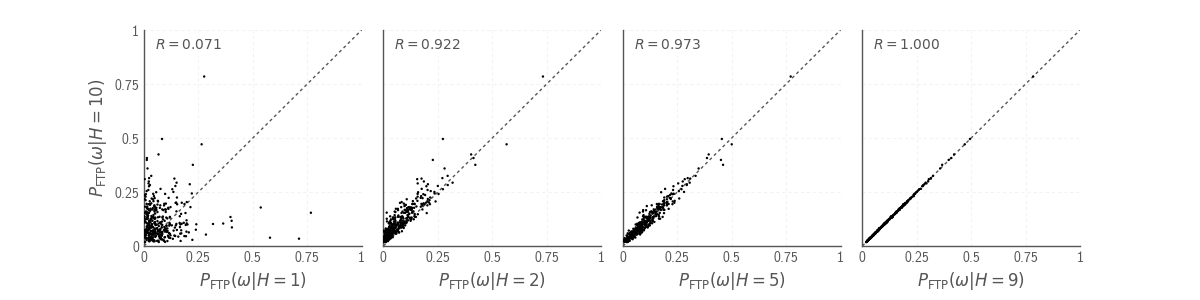
\includegraphics[width=\textwidth]{plots/correlation_with_large_H.png}
    \caption{\label{fig:corrwhighh} Comparing the template periodogram calculated with $H=10$ harmonics
            to the template periodogram using a smaller number of harmonics $H < 10$. The template and
            data used to perform the periodogram calculations are the same as those shown in Figure \ref{fig:tempsandpdgs}.}    
\end{figure*}

Gatspy uses non-linear optimization at each trial frequency to solve
for the best-fit amplitude, phase, and offset of the template. For
weak signals or signals folded at the incorrect trial period, there
may be a large number of local $\chi^2$ minima in parameter space, and thus
the optimization algorithm may have trouble finding the global minimum. The 
FTP, on the other hand, solves for the optimal parameters directly, and
thus is able to recover optimal solutions even when the signal is weak
or not present.

Figure \ref{fig:corrwgats} illustrates the accuracy improvement with FTP.
For large $P_{\rm FTP}(\omega)$, Gatspy and FTP agree well, while for
$P_{\rm FTP} \lesssim 0.25$, FTP consistently finds better template fits
than Gatspy. For many trial frequencies, Gatspy returns a periodogram value
of $P_{\rm gatspy} = 0$, indicating no improvement over a constant fit,
while FTP is able to find superior solutions at many of these frequencies.

Figure \ref{fig:corrwhighh} compares FTP results obtained using the full template
$(H=10)$ with those obtained using smaller numbers of harmonics. The left-most
plot compares the $H=1$ case (weighted Lomb-Scargle), which, as also demonstrated
in Figure \ref{fig:tempsandpdgs}, illustrates the advantage of the template
periodogram for known, non-sinusoidal signal shapes.


\subsubsection{Computation time}

\begin{figure}
    \centering
    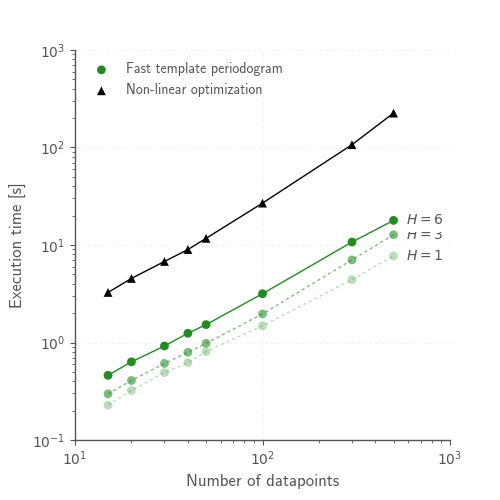
\includegraphics[width=0.5\textwidth]{plots/timing_vs_ndata.png}
    \caption{\label{fig:timingndata} Computation time of FTP compared with Gatspy. For a 6-harmonic
             template and 15 observations, the FTP is three times faster than 
             Gatspy. FTP scales roughly as $\bigO(N)$ (or, for large enough values
             of $N$, $\bigO(N\log N)$), while Gatspy scales as $N^2$, thus the speedup of FTP
             over Gatspy scales linearly in $N$. For large time series of $N\approx 10,000$,
             FTP offers over three orders of magnitude speedup over Gatspy.}
\end{figure}

FTP scales asymptotically as $\bigO(N_fH\log N_fH)$, however the computational
time is usually dominated by computing polynomial coefficients and zero-finding,
which scales as $\bigO(N_f H^4)$, even for very large numbers of frequencies
$(N_f > 10^7)$. 

Figure \ref{fig:timingndata} shows that FTP achieves a factor of 3 speedup for
even the smallest test case (15 datapoints), while for larger cases ($N\sim10^4$)
FTP offers 2-3 orders of magnitude speed improvement over Gatspy. 

\section{Discussion}\label{sec:discussion}

Template fitting is a powerful technique for accurately recovering
the period and amplitude of objects with \emph{a priori} known
lightcurve shapes. It has been used in the literature by, e.g.
\cite{Sesar_etal_2016, Sesar_etal_2010}, to analyze RR Lyrae in the
SDSS and PS1 datasets, where it has been shown to produce purer
samples of RR Lyrae at a given completeness. The computational
cost of current template fitting algorithms, however, limits their
application to larger datasets or with a larger number of templates.

We have presented a novel template fitting algorithm that extends
the Lomb-Scargle periodogram \citep{Lomb_1976,Scargle_1982,Barning_1963,Vanicek_1971}
to handle non-sinusoidal signals that can be expressed in terms of
a truncated Fourier series with a reasonably small number of harmonics
($H\lesssim 10$). 

The fast template periodogram (FTP) asymptotically scales as 
$\bigO(N_fH\log N_fH)$, while previous template fitting algorithms
such as the one used in the \texttt{gatspy} library \citep{gatspy},
scale as $\bigO(N_{\rm obs}N_f\sim N_f^2)$. However, the FTP effectively
scales as $\bigO(N_fH^4)$, since the time needed to compute polynomial
coefficients and perform zero-finding dominates the computational time
for most practical cases ($N_{\rm obs}\sim N_f \lesssim 10^7$).
This effectively restricts the space of templates to those that are
sufficiently smooth to be explained by a small number of Fourier terms.

FTP also improves the accuracy of previous template fitting algorithms, 
which rely on non-linear optimization at each trial frequency to minimize
the $\chi^2$ of the template fit. The FTP routinely finds superior fits,
especially when the signal is weak.

An open-source Python implementation of the FTP is available at
GitHub.\footnote{\url{https://github.com/PrincetonUniversity/FastTemplatePeriodogram}} 
The current implementation can be improved in several ways:

\begin{enumerate}
    \item Improving the speed of the polynomial
          coefficient calculations and the zero-finding steps.
    \item Porting FTP to C/C++ and using CUDA to exploit GPU parallelism.
    \item Extending the FTP to a multi-band periodogram to improve performance
          on sparsely sampled multiband data (e.g. SDSS, LSST, Pan-STARRS).
\end{enumerate}

\begin{table}
\centering
\begin{tabular}{l|l|l|l}
Survey     & $N_{\rm LC}$ & $N_{\rm obs}$ & Refs. \\
\hline\hline
CoRoT      & $1.5\times 10^5$  &  53,000       &       \\
\hline
ASAS-3     &   $2\times 10^7$  &  500          &       \\
\hline
HATNet     & $5.6\times 10^6$  &  10,000       &       \\
\hline
Gaia       &           $10^9$  &  70           &       \\
\hline
SuperWASP  & $3.2\times 10^7$  &  13,870       &       \\
\hline
OGLE-IV    &           $10^9$  &  5000         &       \\
\hline
LSST       & $3.7\times 10^10$ &  825          &       \\
\hline
\end{tabular}
\caption{\label{tab:surveypars} Survey parameters used for Figure \ref{fig:surveys}.
\todo{Add references (if we decide to keep this figure)}}
\end{table}

\begin{figure}
\centering
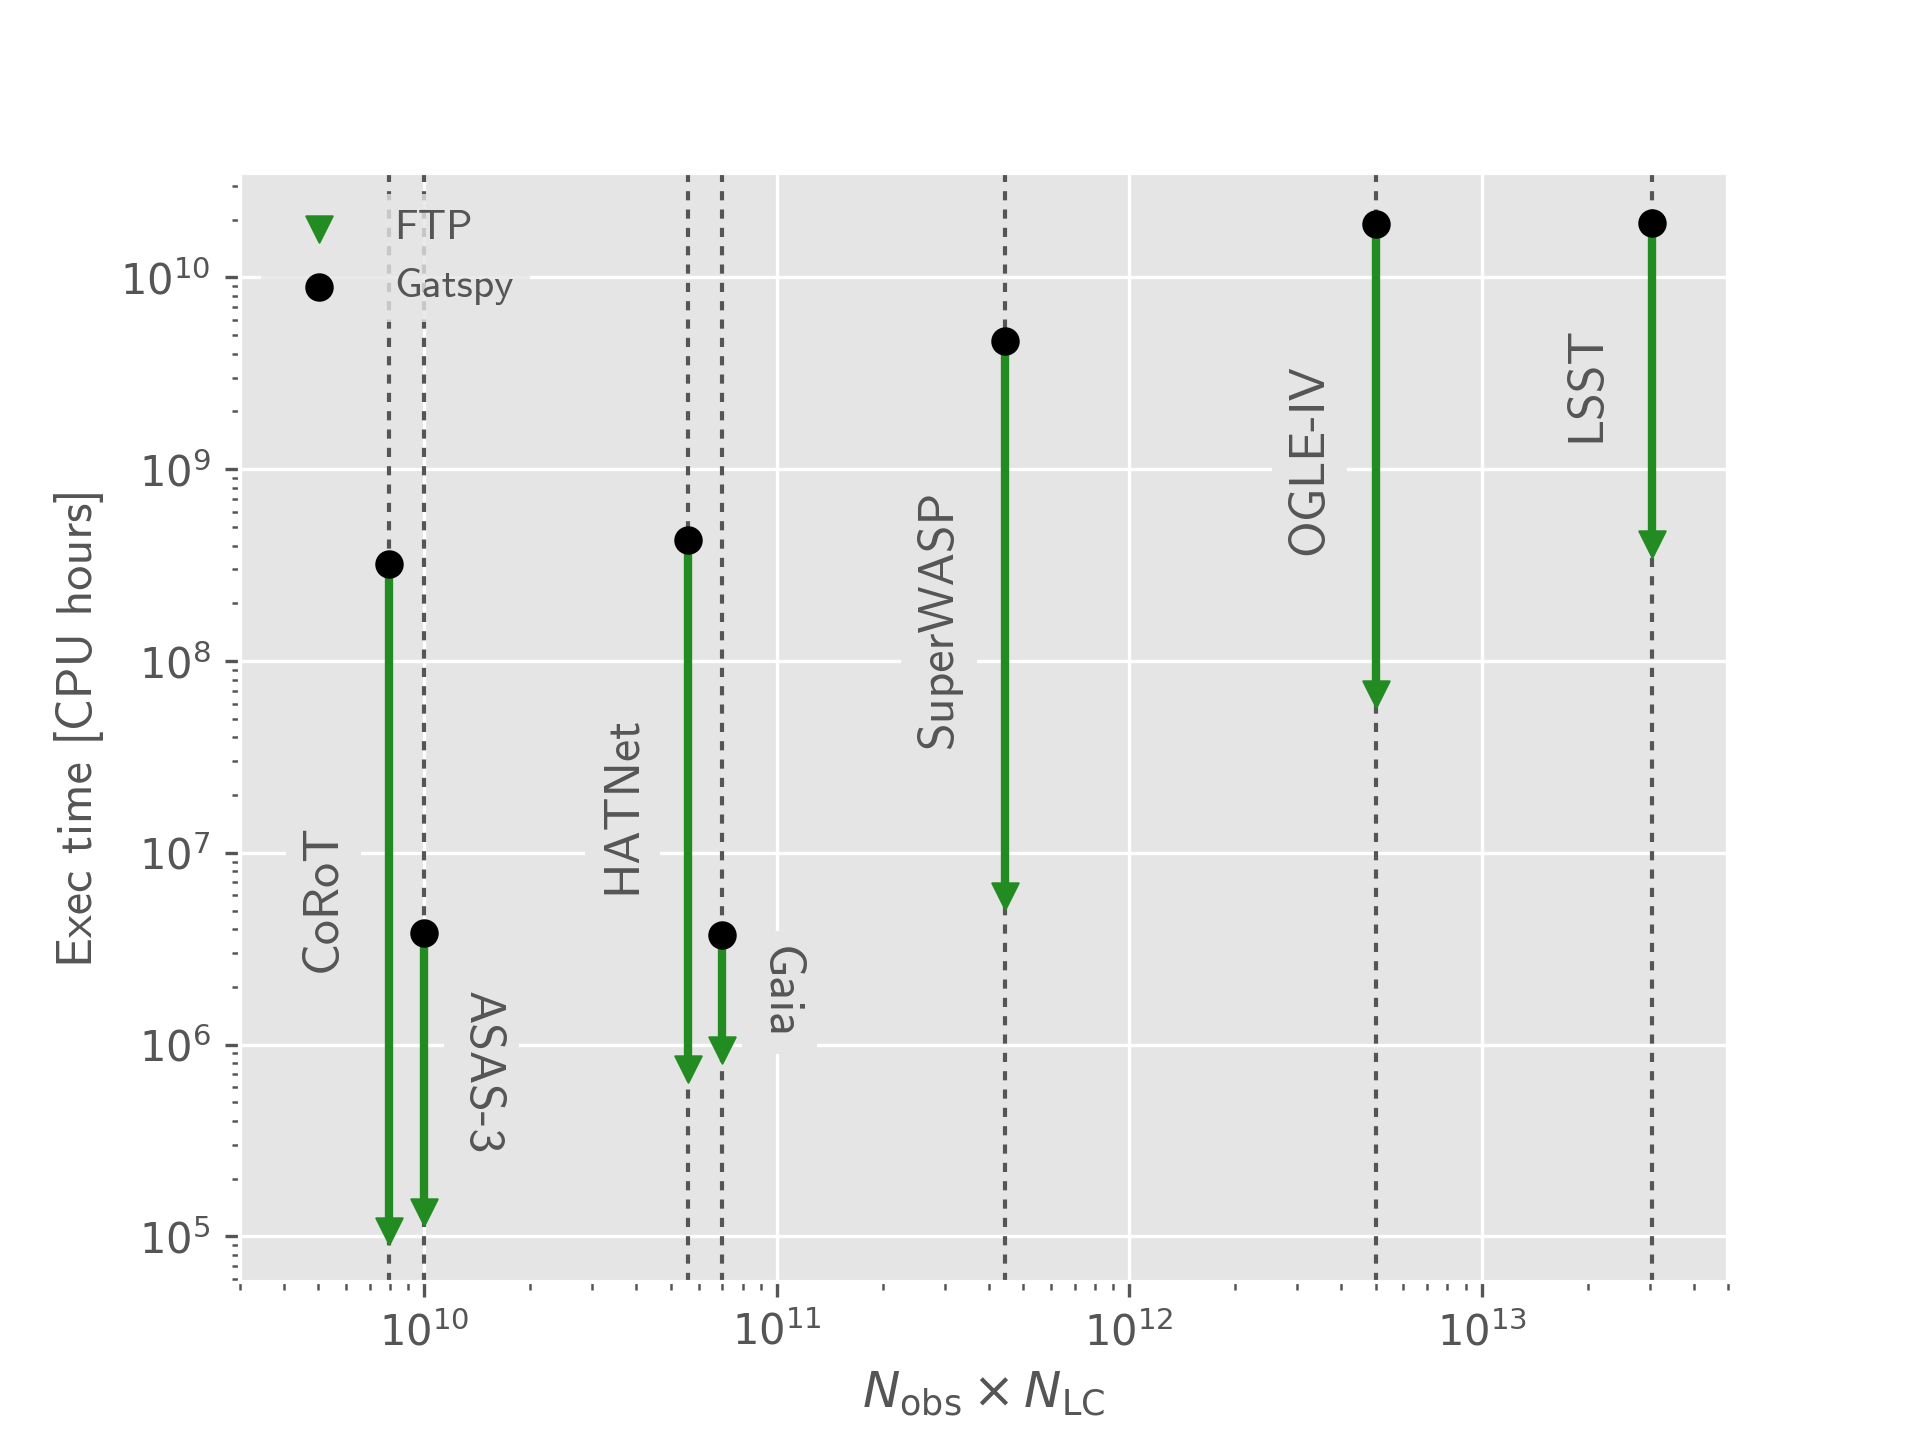
\includegraphics[width=0.5\textwidth]{plots/timing_for_various_surveys.png}
\caption{\label{fig:surveys} Computational resources needed for performing 
a single template periodogram ($H=6$) on an entire survey dataset. Our
python implementation of FTP improves computational efficiency of template 
searches by orders of magnitude in most cases, and in one case by over 
three orders of magnitude (CoRoT). Parameters for $N_{\rm obs}$ and $N_{\rm LC}$
were estimated from publicly available information (see text).}
\end{figure}

As pointed out in \cite{Vanderplas+Ivezic_2015}, current template fitting
procedures are too slow to be practical for LSST-sized time-domain surveys.
We attempt to quantify the improvement in computational efficiency for
several important time-domain surveys, using estimated survey values for 
$N_{\rm obs}$, the number of observations per object, and $N_{\rm LC}$, 
the number of objects with lightcurves in the survey. 

Figure \ref{fig:surveys} shows estimated computation time for a single
template periodogram performed on the entirety of a given survey. For all
surveys, the FTP improves computational efficiency in one case over
three orders of magnitude, but typically between 2-3 orders of magnitude.
Improving the existing implementation, and porting to C/C++ and CUDA,
should further improve these numbers.

Template fitting remains prohibitvely slow for practical applications to
large time-domain surveys, but this work presents a possible shortcut
that potentially could make template fitting a fast and valuable tool.

%Appendix: Proof that GLS is recovered when H=1
\begin{acknowledgements}
\todo{(acknowledge GRANTS.)}
\end{acknowledgements}

\bibliography{refs}
\end{document}
